\documentclass[12pt, a4paper]{article}

\usepackage[hmargin=2.5cm, vmargin=2cm]{geometry}
\usepackage{amsthm, amssymb, mathtools, yhmath, graphicx}
\usepackage{fontspec, type1cm, titlesec, titling, fancyhdr, tabularx}
\usepackage{color}
\usepackage{unicode-math}
\usepackage{float}
\usepackage{hhline}
\usepackage{comment}
\usepackage{siunitx}
\usepackage{csvsimple}
\usepackage{subcaption}

\usepackage[CheckSingle, CJKmath]{xeCJK}
\usepackage{CJKulem}
\usepackage{enumitem}
\usepackage{tikz}
\usepackage[siunitx]{circuitikz}
\usepackage{wrapfig}
%\setCJKmainfont[BoldFont=cwTex Q Hei]{cwTex Q Ming}
%\setCJKsansfont[BoldFont=cwTex Q Hei]{cwTex Q Ming}
%\setCJKmonofont[BoldFont=cwTex Q Hei]{cwTex Q Ming}
\setCJKmainfont[BoldFont=cwTeX Q Hei]{cwTeX Q Ming}

\def\normalsize{\fontsize{12}{18}\selectfont}
\def\large{\fontsize{14}{21}\selectfont}
\def\Large{\fontsize{16}{24}\selectfont}
\def\LARGE{\fontsize{18}{27}\selectfont}
\def\huge{\fontsize{20}{30}\selectfont}

%\titleformat{\section}{\bf\Large}{\arabic{section}}{24pt}{}
%\titleformat{\subsection}{\large}{\arabic{subsection}.}{12pt}{}
%\titlespacing*{\subsection}{0pt}{0pt}{1.5ex}

\parindent=24pt

\DeclarePairedDelimiter{\abs}{\lvert}{\rvert}
\DeclarePairedDelimiter{\norm}{\lVert}{\rVert}
\DeclarePairedDelimiter{\inpd}{\langle}{\rangle}
\DeclarePairedDelimiter{\ceil}{\lceil}{\rceil}
\DeclarePairedDelimiter{\floor}{\lfloor}{\rfloor}

\newcommand{\unit}[1]{\:(\text{#1})}
\newcommand{\df}[1]{\mathop{}\!\mathrm{d^#1}}
\newcommand{\img}{\mathrm{i}}

\title{ \bf {\Huge 電子電路實驗7:雙極非線性元件特性曲線之簡單測量}\\ 實驗結報}
\author{B02901178 江誠敏}

\begin{document}

\maketitle


\section{實驗結果}
由於數據眾多,因此直接以圖表方式呈現。
\subsection{Inverting}
\begin{figure}[H]
  \centering
  \begin{subfigure}[b]{0.45\textwidth}
    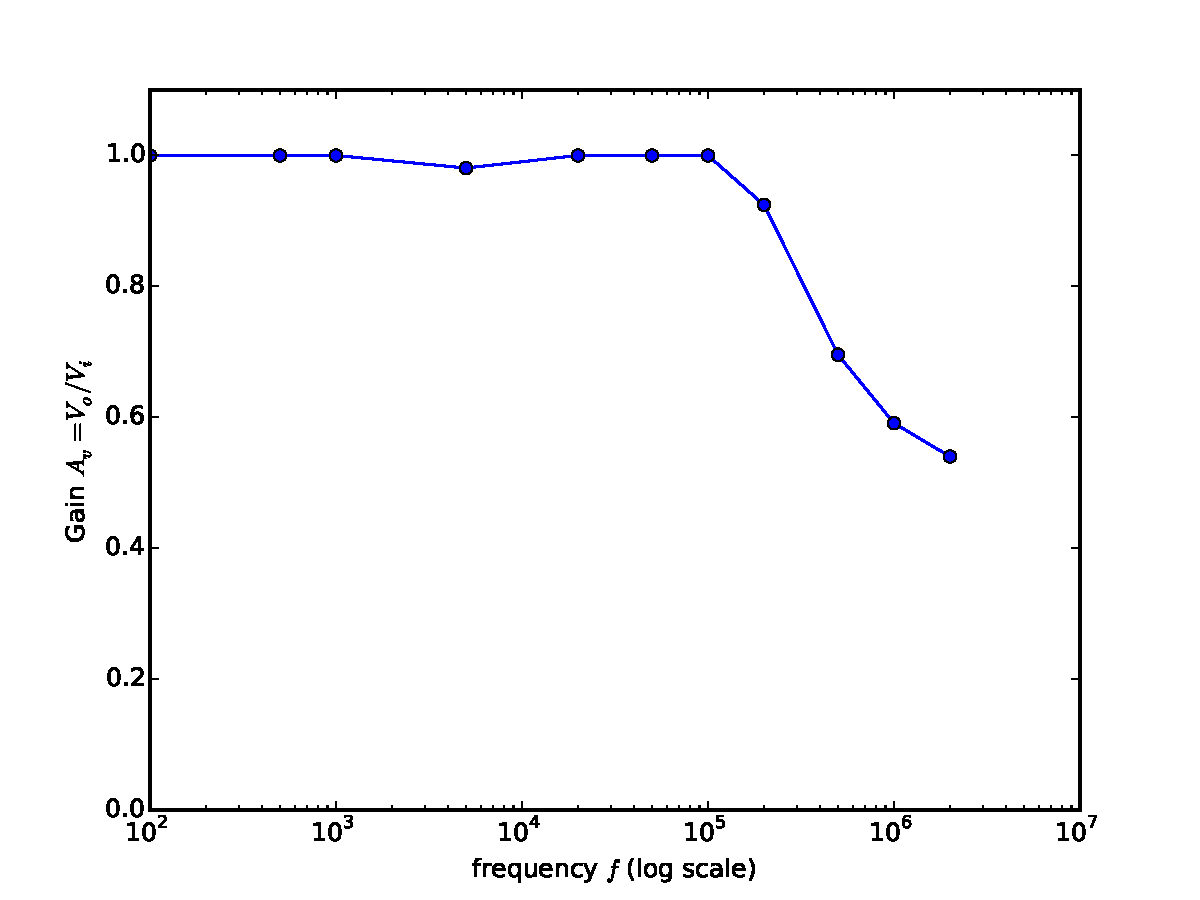
\includegraphics[width=1\textwidth]{img/q1.pdf}
    \caption{\SI{100}\ohm}
  \end{subfigure}
  ~
  \begin{subfigure}[b]{0.45\textwidth}
    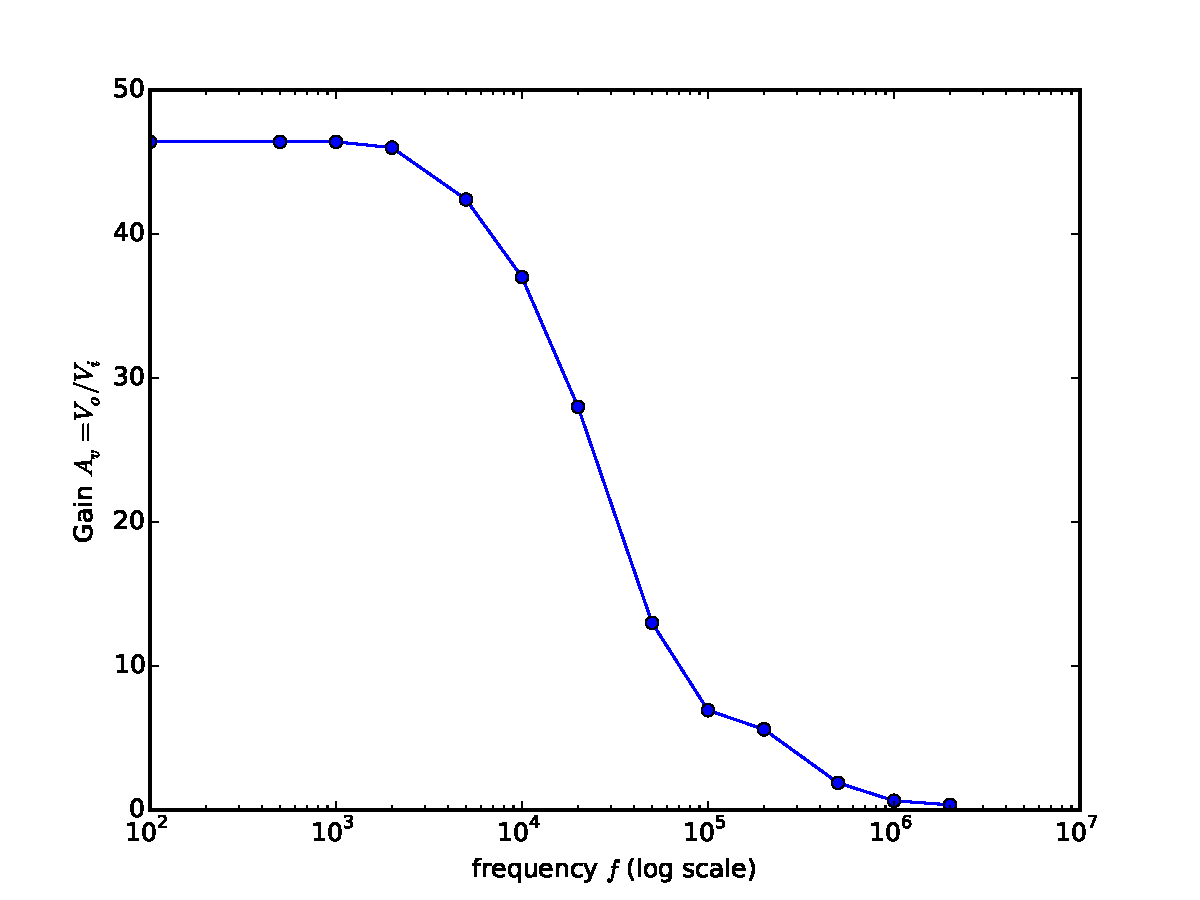
\includegraphics[width=1\textwidth]{img/q2.pdf}
    \caption{\SI{4.7}\kohm}
  \end{subfigure}
\end{figure}

\subsection{Non-Inverting}
\begin{figure}[H]
  \centering
  \begin{subfigure}[b]{0.45\textwidth}
    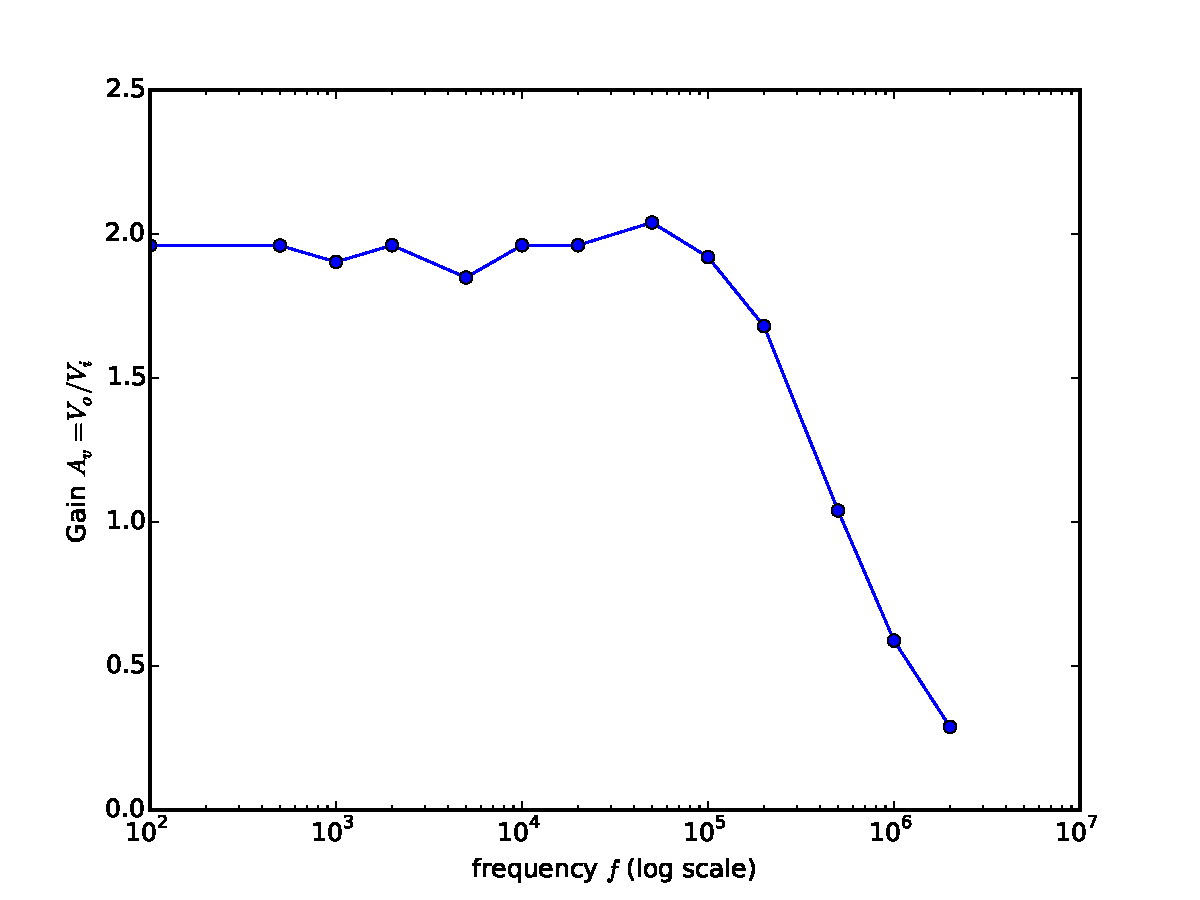
\includegraphics[width=1\textwidth]{img/q4.pdf}
    \caption{\SI{100}\ohm}
  \end{subfigure}
  ~
  \begin{subfigure}[b]{0.45\textwidth}
    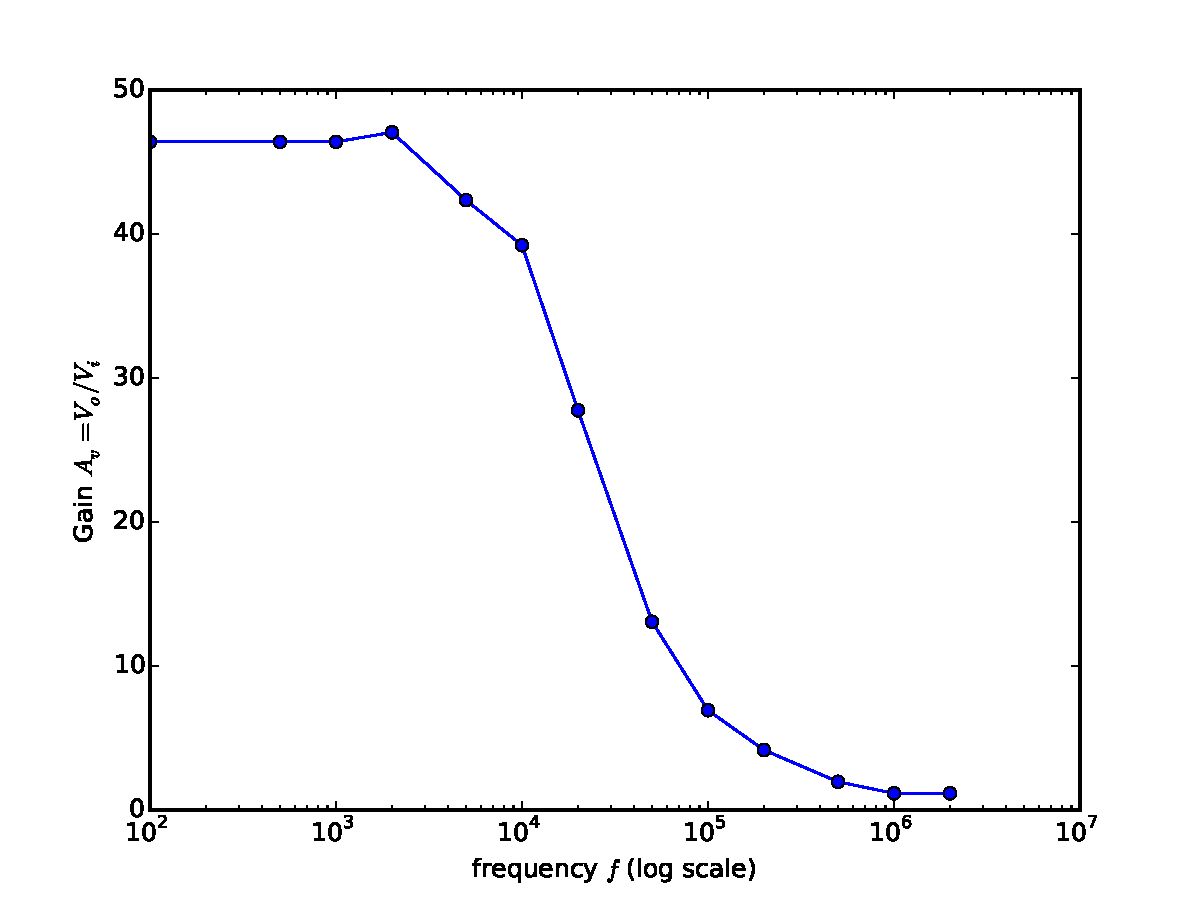
\includegraphics[width=1\textwidth]{img/q3.pdf}
    \caption{\SI{4.7}\kohm}
  \end{subfigure}
\end{figure}

\subsection{Follower}
\begin{figure}[H]
  \centering
  \begin{subfigure}[b]{0.45\textwidth}
    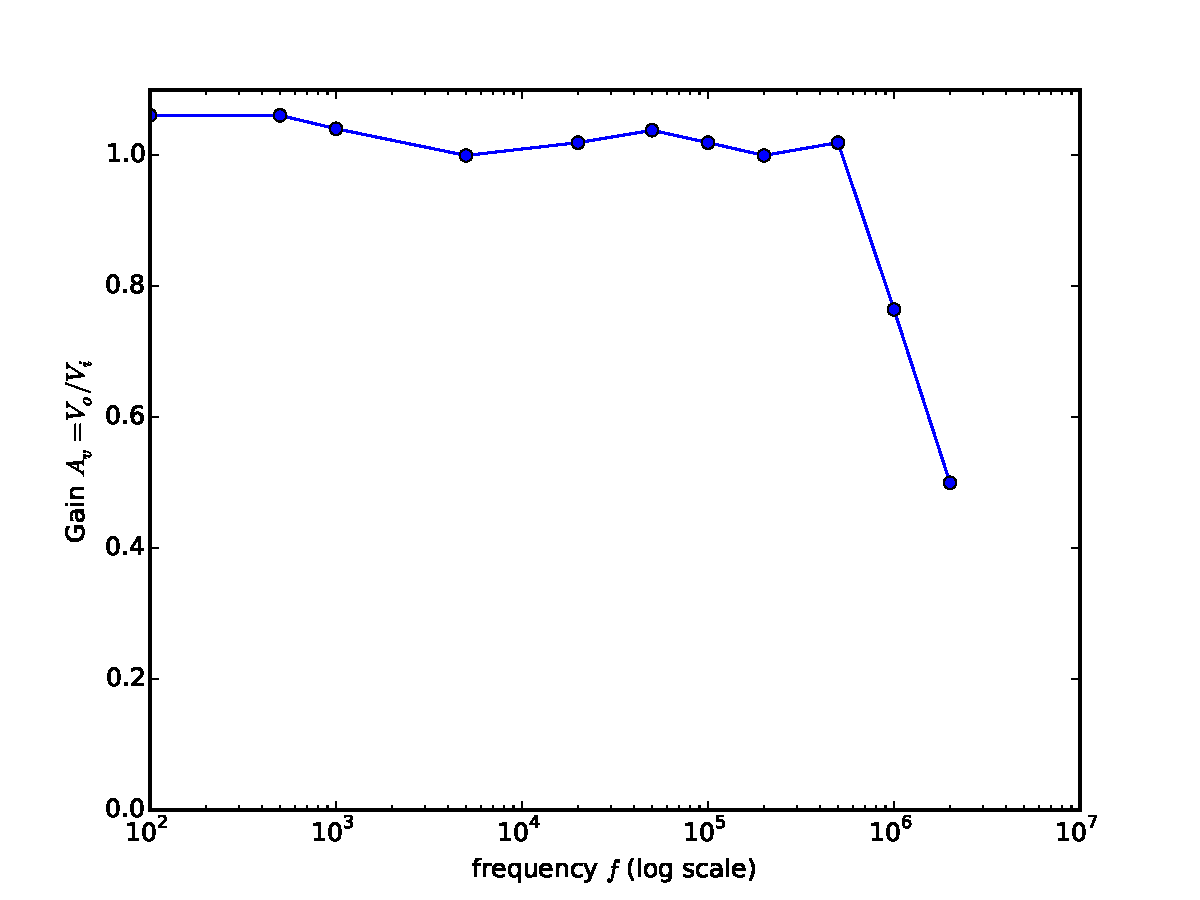
\includegraphics[width=1\textwidth]{img/q5.pdf}
  \end{subfigure}
\end{figure}



\section{結報問題}

\begin{enumerate}[itemsep=20pt, topsep=10pt]
  \item {\large\bf 何謂 common-mode rejection ratio (CMRR)?對放大電路有何重要性?} \\[10pt]
    答:\\
    對於一個 Two input terminals, one output terminal的線性電路,我們可以將輸出電壓寫成
    \[ V_o = C_1 V_1 + C_2 V_2 \]
    而這個式子又可以再進一步寫成
    \[ V_o = A_d (V_1 - V_2) + \frac{1}{2} A_{cm} (V_1 + V_2) \]
    其中$A_d$就是Difference gain, 而$A_{cm}$就是Common mode gain。可以想作$A_{cm}$是當兩端電壓相同時─也就是共同訊號─的放大倍率。而$A_d$就是兩端電壓差被放大的倍率。
  我們定義 \[ \text{CMRR} \equiv 10 \log \frac{A_{d}}{A_{cm}} \]
  因為在現實中,通常兩個輸入端都會在一個Voltage Bias下運作,所以我們關心的是Difference Gain的大小,而非Common mode gain的大小。並且如果Common mode gain太大,還可能使輸出電壓超過放大器的上限。因此我們會希望$A_d$越大,$A_{cm}$越小越好,而這個性質恰好可以用CMRR來衡量。理論上我們會希望CMRR越大越好!

\item {\large\bf 何謂 gain bandwidth product (GBP)?根據實驗數據,μA741 的 GBP 是多少?請寫出計算過程。} \\[10pt]
  一般一個放大器的放大倍率可以用下列式子描述:
  \[ A(\omega) = \frac{A_0}{\sqrt{1 + \left( \frac{\omega}{\omega_c} \right)^2 }} \]
  其中$\omega_c$為3-db frequency。當$\omega \gg \omega_c$時,有
  \[
  A(\omega) \approx \frac{A_0}{\frac{\omega}{\omega_c}} = \frac{A_0 \omega_c}{\omega} \]
  所以
  \[
  A(\omega) \omega \approx A_0 \omega_c, \quad \text{if } \omega \gg \omega_c \]
  也就是Gain 和 "Bandwidth" 的乘積差不多是個定值!我們就定義此值為Gain bandwidth product。
  而要計算uA741的bandwidth product,我們先選一個適當的$A(\omega)$(不可太大),再回堆$\omega$,最後計算$A(\omega) \omega$。就拿Inverting $\SI{100}\ohm$當例子。為了方便我們不妨令$A(\omega) = 1$,接著我們計算此時的$V_o / V_i$為多少($V_o / V_i$不見得等於$A(\omega)$!),可以列出
  \[
    A(\omega) \left(0 - \frac{V_o + V_i}{2}\right) = V_o \; \Rightarrow \; V_o = \frac{-1}{3} V_i
  \]
  因此我們對表找什麼時後$V_o / V_i$降到$1/3$就可以知道答案!
  而當然,我們可以選則用Inverting $\SI{4.7}\kohm$比較好算,在$A(\omega) = 1$時
  \[
    A(\omega) \left(0 - \frac{V_o + 47 V_i}{48}\right) = V_o \; \Rightarrow \; V_o = \frac{-47}{49} V_i \approx V_i
  \]
  因此我們找到$V_o / V_i = 1$的頻率,用內差法差不多是$\SI{8.5e5}\Hz$,所以$\text{GBP} \approx \SI{8.5e5}{} \cdot 1 \approx \SI{8.5e5}{}$
  \begin{figure}[H]
    \centering
    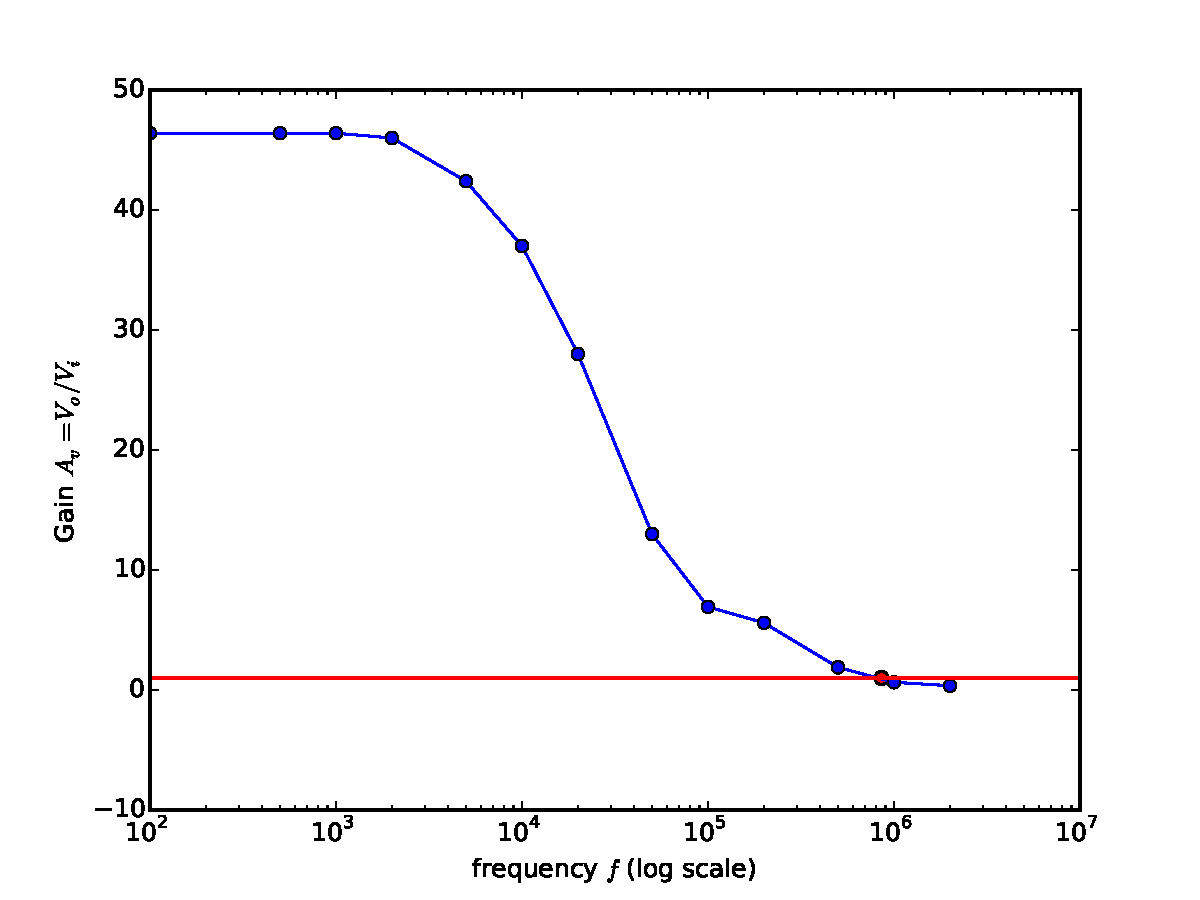
\includegraphics[width=0.6\textwidth]{img/r1.pdf}
  \end{figure}

  \item {\large\bf 在增益同樣為 1 的情況下,反相放大器與電壓隨耦器何者頻寬較大?為什麼?} \\[10pt]
    同上一題的計算方式,不妨都假設$A(\omega) = 1$,此時反相放大器在上一題已經計算過,倍率為$-1/3$,而對於Follower:
    \[
      A(\omega) (V_i - V_o) = V_o \; \Rightarrow V_o = \frac{1}{2} V_i
    \]
    因此反相的GBP為$\frac{1}{3} \omega$,Follower為$\frac{1}{2} \omega$,所以Follower的頻寬較大!與實驗的結果相符。
  \item {\large\bf 實驗中 vi的峰對峰值為 100mV,是否可以改用 1V?為什麼?} \\[10pt]
    最好不要!因為在Inverting $\SI{4.7}\kohm$的輸出放大倍率為$47$倍,如果用$\SI{1}\V$,表示輸出電壓可達到$\SI{47}\V$,遠超過供給電壓$V_{\text{CC}} = \SI{15}\V$!
  \item {\large\bf 實際的運算放大器,其開路 3dB 頻寬(open-loop 3dB-bandwidth)都非常小,這非常小的頻寬的現象其實是刻意要這樣設計的,為什麼?} \\[10pt]
    根據第二題,$A_0 \omega_c = \text{const}$,其中$A_0$是在低頻的放大倍率,$\omega_c$是3db frequency。但運算放大器的開路放大倍率通常都要非常大,作為犧牲,$\omega_c$就只能小囉。 
\end{enumerate}

\section{心得}
這次的實驗真的是燒uA741大賽,因為有說如果燒壞的話,成績就從B起跳,因此我一開始都不太敢亂動,不過才沒多久,四處早已是IC燒焦的味道。就看到旁邊的人急急忙忙在搧風,然後趕緊去找多的uA741。其實後來發現線路不要接錯,電源慢慢從小開到大,似乎也沒那麼容易燒壞uA741。
\end{document}

